\chapter{Analysis and specification of requirements}
\minitoc
\newpage

\setcounter{secnumdepth}{0} % Set the section counter to 0 so next section is not counted in toc
% ----------------------- Introduction ----------------------- %
\section{Introduction}
In this chapter, we are going to analyze the various specifications and requirements of the whole ILG project from development to production.
We will also describe the product's main features and the conception that should be met for the end result.

\setcounter{secnumdepth}{2} % Resume counting the sections for the toc with a depth of 2 (Sections and sub-sections)
% ----------------------- Functional Requirements ----------------------- %
\section{Functional requirements}
Since our project is fairly voluminous, we identify what we consider the necessities for ILG as follows:
\begin{itemize}
	\item Actively editing and enhancing the portal server dashboard by implementing new features to increase customer satisfaction.
	\item Separating the monolithic application to multiple microservices to validate the \glsxtrfull{poc} as instructed by our Product Owner before proceeding with the making of the new architecture.
	\item Daily monitoring of the old system by reading logs directly from the server.
	\item Ensuring that the lead generating is happening in the background with the newly implemented microservices architecture.
	\item Creating individual Dockerfiles for all microservices based on what they require.
	\item Creating the GitLab CI pipelines for all microservices and configuring them to build and push Docker images.
	\item Creating a custom configurable Helm Chart for the whole ILG application stack.
	\item Working on the CD part of the pipelines by setting up a clear deployment strategy to Kubernetes using the custom Helm Chart.
	\item Setting up modern monitoring solutions that use the most out of our Kubernetes deployment with the most recent tools on the market.
\end{itemize}

\subsection{Application dashboard}

\subsubsection*{\underline{Use case}}
We use the Unified Modeling Language (UML) to describe the behavior of the system.
\begin{figure}[H]
	\centering
	\makebox[\textwidth]{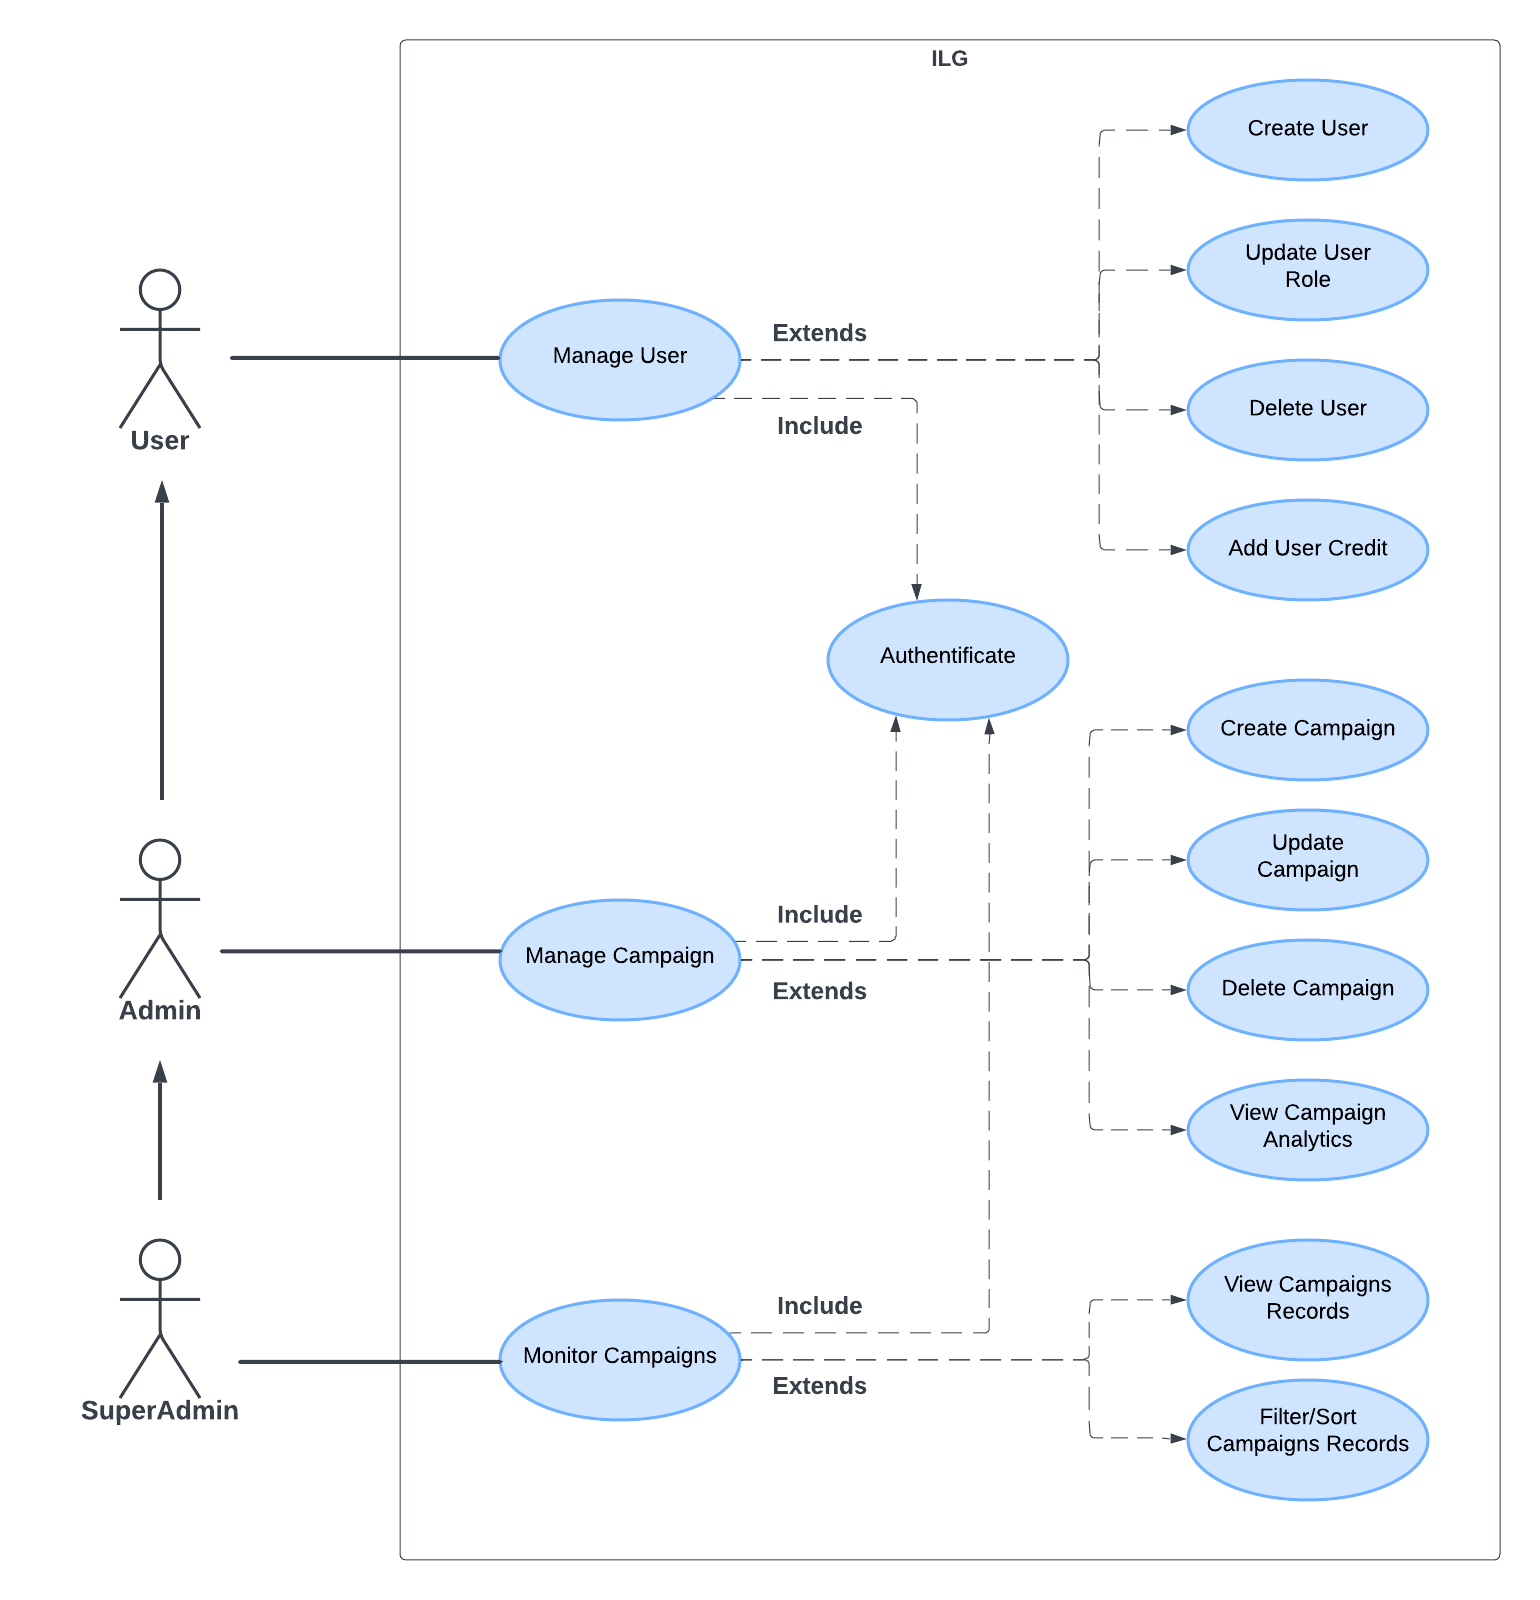
\includegraphics[width=\linewidth]{src/assets/diagrams/usecase.png}}
	\caption{Use case diagram for the frontend dashboard}
	\label{fig:use-case-diagram}
\end{figure}

\subsubsection*{\underline{Actors}}
Mainly, there are 3 types of actors of the system:
\begin{itemize}
	\item \textbf{Super Admin}: The main administrator with full access permissions to the system.
	\item \textbf{Admin:} The administrator of the system with slightly less privileges than the Super Admin.
	\item \textbf{User:} The main user of the system, who benefits from the different features the system offers, usually a client representative.
\end{itemize}

\subsubsection*{\underline{User management}}
Here are the main requirements of user management for the different type of actors:
\begin{itemize}
	\item As a \textbf{Super Admin}, I can create, modify or delete users and admins accounts.
	\item As an \textbf{Admin}, I can create, modify or delete user's accounts (clients).
	\item As an \textbf{Admin}, I can add or remove credit from user's accounts (clients).
	\item As an \textbf{Admin}, I can view my user's accounts, their used and bought credits.
\end{itemize}

\subsubsection*{\underline{Campaign management}}
Here are the main requirements of campaign management for the different type of actors:
\begin{itemize}
	\item As a \textbf{User}, I can create my campaign specifying the LinkedIn account credentials to be used, the campaign list, salutation messages, invite messages, follow up messages and the number of invites per day.
	\item As a \textbf{User}, I can update my campaigns details such as the LinkedIn account credentials, the campaign list, salutation messages, invite messages, follow up messages and the number of invites per day.
	\item As a \textbf{User}, I can delete my campaigns.
	\item As a \textbf{User}, I can activate my campaigns.
	\item As a \textbf{User}, I can stop my campaigns.
	\item As a \textbf{User}, I can export information about the scraped leads as a CSV file.
\end{itemize}

\subsubsection*{\underline{Campaign monitoring}}
\begin{itemize}
	\item As a \textbf{Super Admin}, I can view the campaigns' records, on day by day basis or in a specific range of dates with information such as number of invites sent, number of follow ups sent and the number of withdrawn invites.
	\item As a \textbf{User}, I can view my campaigns' analytics with information such as requested, connected, replied leads, and conversion rates.
\end{itemize}

\subsection{Lead generating}

\subsubsection*{\underline{Definition}}
The lead generating is the process of \textbf{scraping} the LinkedIn accounts and \textbf{generating} leads by sending them customized invites and follow ups messages through the LinkedIn UI depending on the user's campaign preferences.
So here is the requirements of both parts:

\subsubsection*{\underline{Scraping leads}}
\begin{itemize}
	\item Each day, the system generates a list of URLs to scrape from a campaign (search) list and saves them as tasks in the database where each list item corresponds to a lead's profile URL.
	\item Each day, the leads' information are scraped from the previously generated URLs. Each scraped URL corresponds to one lead and is saved as an entry in the database.
\end{itemize}

\subsubsection*{\underline{Generating leads}}
\begin{itemize}
	\item Each day, the system sends a certain number of invites to the scraped leads. The number is between a range the user specifies in the UI.
	\item The system sends out the first follow up message to leads that accepted the connection request but did not yet reply. The first follow up message is sent at the earliest 24 hours after the connection request has been sent.
	\item The second follow up message is sent out on the day after the first follow up message was sent if the lead did not reply yet.
\end{itemize}

\newpage

% ----------------------- Conception ----------------------- %
\section{Conception}
In this section, we will dive deep into the conception and the logic behind the parts of the application:

\subsection{Architecture}
The next diagram shows the various microservices that make up our application.
The bulleted lists show the main tasks of each of the services.
We can see that the heavy services interact with a GraphQL data layer whereas the frontend interacts with an API layer.

We will discuss each service with more details in the upcoming sub-sections.

\begin{figure}[H]
	\centering
	\makebox[\textwidth]{\includegraphics[width=15cm]{src/assets/diagrams/overview.png}}
	\caption{Overview of ILG services}
	\label{fig:services-overview}
\end{figure}

\subsubsection*{\underline{Microservices}}
\begin{table}[H]
	\renewcommand{\arraystretch}{1.5}%
	\caption{All the application's Microservices}
	\centering
	\medskip
	\begin{tabularx}{1\textwidth} {
			| >{\hsize=.8\hsize\linewidth=\hsize\centering\arraybackslash}X
			| >{\hsize=1.75\hsize\linewidth=\hsize\justifying\arraybackslash}X
			| >{\hsize=0.45\hsize\linewidth=\hsize\centering\arraybackslash}X |}
		\hline
		\rowcolor{primary} \textbf{Name} & \noindent \textbf{Description}                                                                                                  & \textbf{Scalable} \\
		\hline
		\textbf {ilg-data}               & \noindent A GraphQL data access layer used to feed all needed data for other services from the PostgreSQL database.             & No                \\
		\hline
		\textbf {ilg-api}                & \noindent A RESTful api used to serve data to the React app dashboard.                                                          & No                \\
		\hline
		\textbf {ilg-front}              & \noindent A React app dashboard application served through NGINX.                                                               & No                \\
		\hline
		\textbf {ilg-scheduler}          & \noindent The service that's responsible for scheduling and orchestrating the tasks queues and notifications.                   & No                \\
		\hline
		\textbf {ilg-scraper}            & \noindent The service that's responsible for scraping leads from the campaign links generated from LinkedIn Sales Navigator.    & Yes               \\
		\hline
		\textbf {ilg-automation}         & \noindent The service that's responsible for handling LinkedIn accounts' inboxes, threads and for sending invites to the leads. & Yes               \\
		\hline
	\end{tabularx}
\end{table}

\subsubsection*{\underline{Cloud Infrastructure}}
Since we are deploying to a Kubernetes cluster, we decided to distribute our different microservices into their corresponding nodes or virtual machines depending on their shared components and scalability.
\begin{figure}[H]
	\centering
	\makebox[\textwidth]{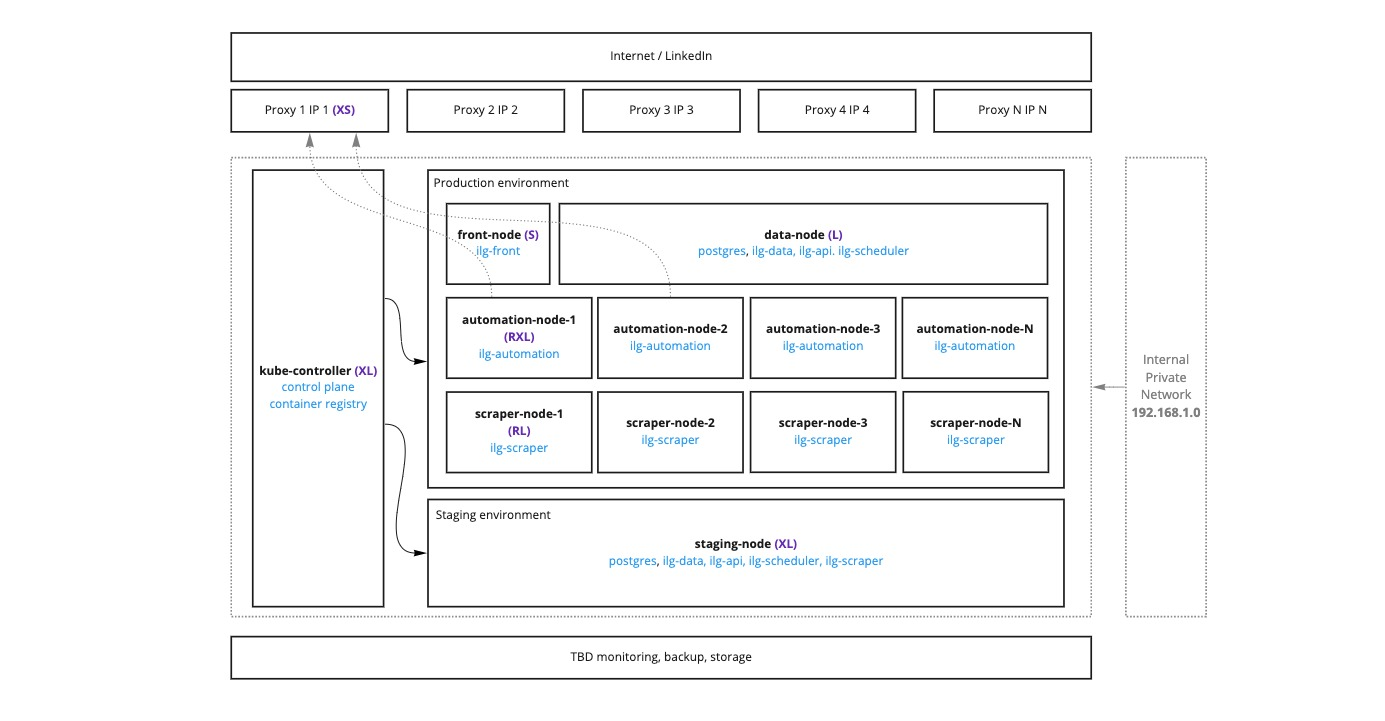
\includegraphics[width=22cm]{src/assets/diagrams/cloud_infra.jpeg}}
	\caption{Cloud infrastructure of the application}
	\label{fig:cloud-infrastructure}
\end{figure}

\subsection{Tasks \& Queues}

\subsubsection*{\underline{In theory}}
Task queues allow services to perform work in the form of asynchronous tasks outside of a user request.
If an app needs to execute work in the background, it adds the tasks it needs to the task queues. The tasks are executed later, by worker services. The Task Queue service is designed for asynchronous work.
Every lead scraping or generating tasks are implemented as a task queue.
\begin{figure}[H]
	\centering
	\makebox[\textwidth]{\includegraphics[width=12cm]{src/assets/diagrams/task-queue.png}}
	\caption{Task queues}
	\label{fig:task-queue}
\end{figure}

\subsubsection*{\underline{Tasks queues types}}
\begin{table}[H]
	\renewcommand{\arraystretch}{1.5}%
	\caption{The application's tasks or jobs}
	\centering
	\medskip
	\begin{tabularx}{1\textwidth} {
			| >{\hsize=0.7\hsize\linewidth=\hsize\centering\arraybackslash}X
			| >{\hsize=1.3\hsize\linewidth=\hsize\justifying\arraybackslash}X |}
		\hline
		\rowcolor{primary} \textbf{Name} & \noindent \textbf{Description}                                                                  \\
		\hline
		\textbf {campaign-scrape}        & \noindent Scrapes a list of leads from a campaign search list or URL.                           \\
		\hline
		\textbf {lead-scrape}            & \noindent Scrapes the lead information from a URL and saves it in the database.                 \\
		\hline
		\textbf {handle-inbox}           & \noindent Opens the conversation inbox of leads and sends them follow up messages if necessary. \\
		\hline
		\textbf {send-invite}            & \noindent Sends a connection invite to leads through LinkedIn.                                  \\
		\hline
	\end{tabularx}
\end{table}

\subsubsection*{\underline{Scheduling tasks}}
Scheduling the different types of tasks is mainly done by the ilg-scheduler service on a daily basis according to a specific cron job we specify in code.
We use the database that's accessible by ilg-data, as the store of those task queues with all of their corresponding information and state.
The diagram below illustrates the different producers and consumers of the tasks in more details.
\begin{figure}[H]
	\centering
	\makebox[\textwidth]{\includegraphics[width=16cm]{src/assets/diagrams/producer_consumer.png}}
	\caption{Diagram detailing the producers and the consumers}
	\label{fig:producer-consumer-diagram}
\end{figure}

\subsection{Scraper \& Automation}
The ilg-scraper and ilg-automation services are responsible for consuming the tasks generated by the system on a daily basis.

The main purposes of the two modules boils down to:
\begin{itemize}
	\item \textbf{Scraper:} Scrapes the LinkedIn information of various leads from a campaign link that is a valid sales navigator URL.
	\item \textbf{Automation:} Generates leads by sending connection requests or invites to the many LinkedIn profiles saved by the scraper using the customer's LinkedIn account.
\end{itemize}

So that in the end, if a lead replies to a customer, we register that as a valid lead that has been acquired and save a new record to be able to accurately bill our customers.

\subsubsection*{\underline{Scraper service flow}}
\begin{figure}[H]
	\centering
	\makebox[\textwidth]{\includegraphics[width=16cm]{src/assets/diagrams/campaign_scraper_sequence.png}}
	\caption{Campaign scraper sequence diagram}
	\label{fig:campaign-scraper-sequence-diagram}
\end{figure}
\begin{figure}[H]
	\centering
	\makebox[\textwidth]{\includegraphics[width=16cm]{src/assets/diagrams/lead_scraper_sequence.png}}
	\caption{Lead scraper sequence diagram}
	\label{fig:lead-scraper-sequence-diagram}
\end{figure}
\newpage

\subsubsection*{\underline{Automation service flow}}
\begin{figure}[H]
	\centering
	\makebox[\textwidth]{\includegraphics[width=16cm]{src/assets/diagrams/send_invite_sequence.png}}
	\caption{Diagram detailing the producers and the consumers}
	\label{fig:send-invite-sequence-diagram}
\end{figure}
\begin{figure}[H]
	\centering
	\makebox[\textwidth]{\includegraphics[width=16cm]{src/assets/diagrams/handle_inbox_sequence.png}}
	\caption{Diagram detailing the producers and the consumers}
	\label{fig:handle-inbox-sequence-diagram}
\end{figure}
\newpage

\subsection{Data Layers}
\subsubsection*{\underline{Schema or Entity Relationship Diagram (ERD)}}
\begin{figure}[H]
	\centering
	\makebox[\textwidth]{\includegraphics[width=16cm]{src/assets/diagrams/er.png}}
	\caption{Entity Relationship Diagram}
	\label{fig:entity-relationship-diagram}
\end{figure}
\newpage

\subsubsection*{\underline{Communication between services}}
For the intra-communication between the various services, two interfaces are provided:
\begin{itemize}
	\item \textbf{GraphQL API Layer:}
	      This interface is used by all the internal services of the application to access the data.
	      In other words, this layer is only reachable within the \textbf{internal private virtual network} and it is \textbf{not exposed publicly}.
	\item \textbf{RESTful API Layer:}
	      This interface is used by the frontend service to access the data. In other words, this layer is \textbf{exposed publicly}.
	      It is of course secured by a JWT token level authentication.
\end{itemize}

% --------------- Non functional Requirements --------------- %
\section{Non-functional requirements}
Non functional requirements describe any specification that does not add direct business value but is nonetheless crucial for the good operation of a developed software.
For \glsxtrshort{ilg}, what we should focus on is:
\begin{itemize}
	\item \textbf{Reliability and Availability:} The software should be available 24 hours a day and 7 days a week.
	\item \textbf{Security:} Clients should be able to safely authenticate to the dashboard with a strong authentication system.
	\item \textbf{Maintainability and Recoverability:} We should respond to LinkedIn changes all the time as fast as possible.
	\item \textbf{Scalability:} This is the main reason we're migrating to a new architecture in the first place.
	\item \textbf{Documentation:} We should always document each and every step we make extensively so that new developers can onboard on the project in a fast and efficient way, which further emphasizes reliability.
\end{itemize}

\setcounter{secnumdepth}{0} % Set the section counter to 0 so next section is not counted in toc
% ----------------------- Conclusion ----------------------- %
\section{Conclusion}
In this chapter, we discussed our main objectives that we should meet during the course of our internship.
We also discuss the various layers and services of the application.
In what follows, we will discuss the realization part with heavy focus on DevOps and the actual implementation of the new architecture.
